\documentclass[10pt]{article}
\usepackage[letterpaper]{geometry}
\geometry{verbose,tmargin=1in,bmargin=1in,lmargin=1in,rmargin=1in}
\usepackage{setspace}
\usepackage{ragged2e}
\usepackage{color}
\usepackage{titlesec}
\usepackage{graphicx}
\usepackage{float}
\usepackage{mathtools}
\usepackage{amsmath}
\usepackage[font=small,labelfont=bf,labelsep=period]{caption}
\usepackage[english]{babel}
\usepackage{indentfirst}
\usepackage{array}
\usepackage{makecell}
\usepackage[usenames,dvipsnames]{xcolor}
\usepackage{multirow}
\usepackage{tabularx}
\usepackage{arydshln}
\usepackage{caption}
\usepackage{subcaption}
\usepackage{xfrac}
\usepackage{etoolbox}
\usepackage{cite}
\usepackage{url}
\usepackage{dcolumn}
\usepackage{hyperref}
\usepackage{courier}
\usepackage{url}
\usepackage{esvect}
\usepackage{commath}
\usepackage{verbatim} % for block comments
\usepackage{enumitem}
\usepackage{hyperref} % for clickable table of contents
\usepackage{braket}
\usepackage{titlesec}
\usepackage{booktabs}
\usepackage{gensymb}
\usepackage{longtable}
\usepackage{listings}
\usepackage{cancel}
\usepackage{tcolorbox}
\usepackage[mathscr]{euscript}
\lstset{
	basicstyle=\ttfamily\small,
    frame=single,
    language=fortran,
    breaklines=true,
    commentstyle=\color{magenta}\ttfamily,
    postbreak=\raisebox{0ex}[0ex][0ex]{\ensuremath{\color{red}\hookrightarrow\space}}
}

% for circled numbers
\usepackage{tikz}
\newcommand*\circled[1]{\tikz[baseline=(char.base)]{
            \node[shape=circle,draw,inner sep=2pt] (char) {#1};}}

\newcommand{\beq}{\begin{equation}}
\newcommand{\eeq}{\end{equation}}
\newcommand{\beqa}{\begin{equation}\begin{aligned}}
\newcommand{\eeqa}{\end{aligned}\end{equation}}

\titleclass{\subsubsubsection}{straight}[\subsection]

% define new command for triple sub sections
\newcounter{subsubsubsection}[subsubsection]
\renewcommand\thesubsubsubsection{\thesubsubsection.\arabic{subsubsubsection}}
\renewcommand\theparagraph{\thesubsubsubsection.\arabic{paragraph}} % optional; useful if paragraphs are to be numbered

\titleformat{\subsubsubsection}
  {\normalfont\normalsize\bfseries}{\thesubsubsubsection}{1em}{}
\titlespacing*{\subsubsubsection}
{0pt}{3.25ex plus 1ex minus .2ex}{1.5ex plus .2ex}

\makeatletter
\renewcommand\paragraph{\@startsection{paragraph}{5}{\z@}%
  {3.25ex \@plus1ex \@minus.2ex}%
  {-1em}%
  {\normalfont\normalsize\bfseries}}
\renewcommand\subparagraph{\@startsection{subparagraph}{6}{\parindent}%
  {3.25ex \@plus1ex \@minus .2ex}%
  {-1em}%
  {\normalfont\normalsize\bfseries}}
\def\toclevel@subsubsubsection{4}
\def\toclevel@paragraph{5}
\def\toclevel@paragraph{6}
\def\l@subsubsubsection{\@dottedtocline{4}{7em}{4em}}
\def\l@paragraph{\@dottedtocline{5}{10em}{5em}}
\def\l@subparagraph{\@dottedtocline{6}{14em}{6em}}
\makeatother

\newcommand{\volume}{\mathop{\ooalign{\hfil$V$\hfil\cr\kern0.08em--\hfil\cr}}\nolimits}

\setcounter{secnumdepth}{4}
\setcounter{tocdepth}{4}

\title{Finite Element Domain Decomposition of the Heat Equation}
\author{April Novak}


\begin{document}
\maketitle

\section{Introduction}

This final project for CS-267 involves the serial creation and parallelization of a finite element solver to the heat equation, which in its simplest form describes the diffusion of temperature with a heat source:

\beq
\label{eq:eq}
-k\frac{\partial^2 T}{\partial x^2}=\dot{q}
\eeq

where \(k\) is the thermal conductivity, \(T\) the temperature, and \(\dot{q}\) a volumetric heat source. This equation is kept very simple so that the goals of the project can focus entirely on parallelization algorithms, rather than more advanced numerical methods for solving convection-diffusion equations that would be encountered in a class such as MATH-228b (Numerical Solutions of Differential Equations). This equation will be solved using domain decomposition (DD) methods in 1-D using MPI for controlling the coarse-grained DD algorithm and OpenMP to obtain fine-grained, loop-level parallelism.

Due to the second derivative present, two boundary conditions are needed (one on each end of the domain). This presents the fundamental difficulty of parallelizing a DD solution - if the domain is divided amongst different parallel processes, then the equations cannot be solved unless guesses are made for the conditions on the interface boundaries that are created upon decomposition. But the solution is not known a priori, so any DD solution will require an iterative procedure, where an initial guess for the interior boundary conditions is continually improved. This application is \textit{not} embarrassingly parallel, and if the number of iterations required to reach convergence is very large, then the parallel runtime can easily be longer than the serial runtime. Hence, clever parallel algorithms will be developed such that a net reduction in runtime and good strong and weak scaling are obtained. The finite element method (FEM) is chosen as the ODE solver because my research focuses on FEM for fluid dynamics applications. The remainder of this section will discuss the numerical method applied to the heat equation in 1-D, and some familiarity with numerical methods is assumed so that the brunt of this report can focus on parallelization. A large fraction of the discussion of the numerical method is deferred to the Appendix, and only the elements necessary to understand the parallel implementation are discussed here (feel free to skip the Appendix). 

The FEM is a weighted residual method that solves the weak form of the governing equation. The weak form is obtained by multiplying Eq. \eqref{eq:eq} by a test function \(\psi(x)\) and integrating over all space:

\beq
\int_{\Omega}\frac{\partial T}{\partial x}k\frac{\partial\psi(x)}{\partial x}dx-\int_{\Gamma}k\frac{\partial T}{\partial x}\psi(x)\cdot\hat{n}dx=\int_{\Omega}\dot{q}\psi(x)dx
\eeq

where \(\Omega\) indicates the entire domain and \(\Gamma\) its boundary. Now, we assume that the numerical solution \(T_h\) is a sum of coefficients multiplied by expansion functions \(\phi\):

\beq
T_h=\sum_{j=1}^{N}c_j\phi_j(x)
\eeq

where there are \(N\) of these expansion functions defined over the domain. The numerical method reduces to the problem of determining the expansion coefficients \(c_j\) for a user-selected set of \(\phi_j(x)\). The Galerkin FEM specifies that \(\psi\) should come from the same space as \(T_h\). Hence, inserting these expansions into the weak form gives a discrete set of matrix equations that can be solved:

\beq
K_{ij}c_j=R_i
\eeq

where the stiffness matrix is:

\beq
\label{eq:k}
K_{ij}=\int_{\Omega}\frac{\partial \phi_j(x)}{\partial x}k\frac{\partial\phi_i(x)}{\partial x}dx-\int_{\Gamma}k\frac{\partial \phi_j(x)}{\partial x}\phi_i(x)\cdot\hat{n}dx
\eeq

and the load vector is:

\beq
R_{i}=\int_{\Omega}\dot{q}\phi_i(x)dx
\eeq

Additional details relating to this weak formulation necessary for numerical implementation, such as quadrature and local-to-global mappings, are contained in the Appendix. In order to solve this discrete system, it is much easier to solve the system over each element individually and then assemble them together into a single, large, matrix system. A connectivity matrix is used to describe how the local element nodes map into the global system. The formation of this connectivity matrix is also contained in the Appendix. 

Once the boundary conditions have been incorporated into the matrix system, as described in the Appendix, the matrix system can be solved by your favorite linear algebra routine. For this assignment, the Conjugate Gradient (CG) method is selected to solve this symmetric system because this will provide more flexibility for exploring parallelization algorithms than simply using some routine from BLAS or LAPACK. To solve a matrix system \(\textbf{K}a=R\) by the CG method requires rewriting the governing equation as the minimization of a potential \(\Pi\). The exact solution is obtained by taking the gradient of this potential with respect to each of the expansion coefficients in the vector \(a\), and setting that gradient equal to zero. The minimizer to the potential \(\Pi\) is also a solution to the matrix system. Details of the CG method are deferred to the Appendix.

This concludes the theoretical discussion of the FEM applied to this simple 1-D heat equation. The next section discusses steps taken to obtain a fast serial implementation of this algorithm, and will go into more detail regarding exactly how this method can be implemented in code. Although the heat equation is only solved in 1-D, no shortcuts are taken with the development of the code. That is, with modifications to the initialization subroutines to set up a mesh and node numberings, I assume nothing about the structure of the matrices or boundary conditions that would invalidate natural extension to higher dimensions (i.e. this assignment could have been much easier had I assumed we would always have a 1-D domain. I ran out of time to extend this to 2-D).

\section{Serial Implementation}

This section discusses the serial code that is used as a launching point for parallelization. As a nuclear engineering student interested in computational methods, you will quickly learn that the consequences of errors in codes used to design nuclear reactors can potentially be very high. Hence, in this field there is very slow acceptance of new modeling codes since each new code must undergo rigorous verification and validation. Many nuclear simulation codes are written in Fortran, so I used this project as an opportunity to learn how to program in Fortran 2003. Psuedo-code for the overall program structure is as follows:

\begin{lstlisting}
! read in problem parameters from command line and namelist
call read_namelist()
call read_commandline()

! initialize problem variables based on user inputs
call initialize_global_mesh()
call define_quadset()
call define_shapefunctions()

! determine elemental matrices
call elementalload()
call elementalstiffness()

! find a good initial guess to serve as input to the CG solver
! ...... discussed later ....... !

! form location matrix
LMfine = locationmatrix(global%n_el, global%n_nodes)

! form global load vector and apply boundary conditions
global%rglob  = globalvector(LMfine, rel, global%n_nodes)

! determine CSR storage of global stiffness matrix
call form_csr(LMfine, global%n_nodes, rows)

! call CG method to solve
solution = conjugategradient(rows, guess, global%rglob, global%BCs)
\end{lstlisting}

Every problem begins by initializing problem variables and determining the elemental matrices. An initial guess is required for the CG solver, and can be as naive as a vector of zeros, or determined in a more fancy way (to be discussed later). Then, the global load vector is formed by looping through the connectivity matrix. The global stiffness matrix is stored in Compressed Sparse Row (CSR) format, to be discussed in the next section. Finally, the CG method is called with the initial guess and the {\tt rows} data structure holding the CSR information. 

\subsection{CSR Format}
An important improvement above the first naive code (not discussed in this report) is the storage of the global stiffness matrix in CSR form. The global stiffness matrix is sparse because we select shape functions that are local, and don't extend over the entire physical domain. With linear elements in 1-D, a maximum of \(4N\) nonzero elements would need to be stored (with \(N\) the number of elements). With a naive implementation, we would store \(N^2\) numbers, but most of them are zero. Hence, the memory improvement associated with implementing CSR storage offers about \(\mathscr{O}(N)\) less storage requirements. The difficulty with implementing CSR storage here is that the structure of the matrix is not known until you actually form the matrix, because there is not a one-to-one correspondence of entries in local matrices to entries in global matrices. That is, some entries overlap due to continuity requirements at inter-element nodes. For instance, in 1-D with linear elements, each element contributes four non-zero numbers to the global stiffness matrix. For \(N\) elements, this amounts to \(4N\) total entries. {\it However}, due to continuity, some entries will overlap (they are added), and the global matrix will only have \(3N-2\) nonzero entries. So how can we use the information in the connectivity matrix to determine which entries of the global matrix result due to a single number, and how many result due to summations of several contributions?

The only way to form the CSR for this application was to determine a relationship between the number of times a node number appears in the connectivity matrix with how many nonzero entries appear on that row in the global matrix. This relationship is different depending on if the mesh is 1-D, 2-D, or 3-D, and on the type of element (2-D triangles vs. 2-D squares), but for 1-D elements, if a node number appears \(n\) times in the connectivity matrix, then that row in the global matrix has \(2(n-1)\) nonzero entries. The CSR storage is formed by looping over the connectivity matrix and counting the number of times each node number appears, and then saving the nonzero values in a vector, and the column numbers corresponding to those nonzero values (which are the entries of the location matrix for that element) in a vector. For an elemental matrix and a location matrix, the {\tt csr\_storage} module assembles the CSR data structure. The runtime associated with this data structure formation is negligible, being less than 0.1\%.

\subsection{Vectorization}

Single Instruction, Multiple Data (SIMD) is the process by which a single instruction is used to perform an operation on multiple pieces of data at the same time. When instructed with the appropriate vectorization flags, the compiler will try to find SIMD parallelism and use them as much as possible. Using the GNU compiler, automatic vectorization can be attempted using the {\tt -O3} flag. For all timing results shown, the {\tt -O3} compiler setting is used. Using this flag, as opposed to zero compiler flags, yields a dramatic performance improvement. The great performance (rather than memory) benefit of the CSR storage is not fully appreciated without an understanding of why some loops cannot be automatically vectorized. If we wanted to avoid the CSR implementation, but still only store the nonzero values of the sparse stiffness matrix, we could implement a different algorithm for sparse matrix-vector multiplication. This requires looping over the location matrix during multiplication according to the following code. Because it is not known {\it which} nodes contribute to the overlapping nodes in the global matrix a priori, this algorithm cannot be vectorized, again due to loop dependence. 

\begin{lstlisting}
result = 0.0
do q = 1, n_el ! loop over the elements
  do i = 1, n_en ! loop over all entries in kel
      do j = 1, n_en ! loop over all entries in kel
        ! loop cannot be vectorized
        result(LM(i, q)) = result(LM(i, q)) + matrix(i, j) * vector(LM(j, q))
      end do
  end do
end do
\end{lstlisting}


\subsection{Scaling}
Because the cost of a matrix-vector product is roughly \(\mathscr{O}(N)\), the cost of the CG solver is \(I\mathscr{O}(n)\), where \(I\) is the number of CG iterations required. However, timing studies show that this routine scales as \(\mathscr{O}(N^2)\), where \(N\) is the size of the matrix. This can be explained by the fact that the CG method is technically a direct method once you perform \(N\) iterations. So, without good preconditioning, the CG method will scale as \(\mathscr{O}(N^2)\). For lack of time, no preconditioning is used in this assignment. About 99.9\% of the runtime is spent in the CG solver for the serial implementation. This will have a dramatic impact on the parallel performance using DD.  


This important feature will be needed to explain the parallel performance observed later.

\section{Parallel Implementation}
This section discusses parallelization of the serial code developed in the previous section. In general, there are two very different parallelization strategies here - the first involves domain decomposition amongst parallel threads, where each parallel thread then runs a complete FEM solution, with iteration between threads until all threads agree on the values of the solution at the boundaries between the domains. Alternatively, a single FEM problem can be run (with no need to iterate boundary conditions because the domain is not decomposed), and the work for the single FEM solve distributed amongst parallel instances. The problem with this second method is that the iterative solution occurs with a {\tt do while} loop, since the iterative solution is continually updated and the number of updates is unknown at runtime. This limits the overall CG solver to serial implementation, so a domain decomposition is more effective so that smaller matrices can be solved with the CG solver. Domain decomposition is also more often used because the domain may be so large and the problem information (such as discretized material properties, multiple components of solution vectors, etc.) so large that it cannot fit into the memory of a single processor. 

There are many variants of domain decomposition algorithms, the earliest being Schwarz methods developed to compare against analytical solutions to differential equations on strange-shaped domains that could be decomposed into simpler shapes. It appears that most domain decomposition methods can be decomposed into two general categories:

\begin{enumerate}
\item Classes with no ``interface'' problem, where the decomposed domains {\it overlap}. The first domain decomposition method developed by Schwarz falls into this category. A 1-D problem can be divided into domains that overlap. Half of the domains solve their domain, using initial guesses for the internal boundary conditions. Then, because the domains overlap, the first half of the domains send a boundary condition value to the second half of domains (indicate with downward blue arrows below), which then solve over their domains individually. This second group then passes updated boundary condition values back to the first group (indicate with upward blue arrows), and iteration continues until convergence. 

\begin{figure}[H]
\centering
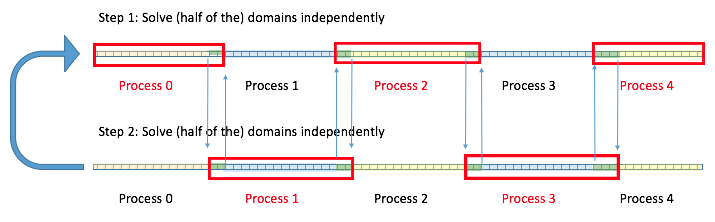
\includegraphics[width=0.8\textwidth]{../figures/1D-schwarz2.png}
\caption{Basic algorithm for 1-D domain decomposition using the overlapping Schwarz method.}
\end{figure}

\item Classes that solve an ``interface problem'' and have no overlapping domains. The union of all the domains equal the original problem dimensions. All locations where boundary conditions are imposed are indicated with vertical red lines. Because the solution is not known a-priori, the boundary conditions on the interior of the domain, between adjacent domains, must be guessed. After each process solves its domain individually, an interface problem is solved between each domain using updated solution values from the most recent domain solve. The interface problem is used to compute an updated domain-interface boundary condition, which is sent back to the individual domains. Iteration continues until convergence.

\begin{figure}[H]
\centering
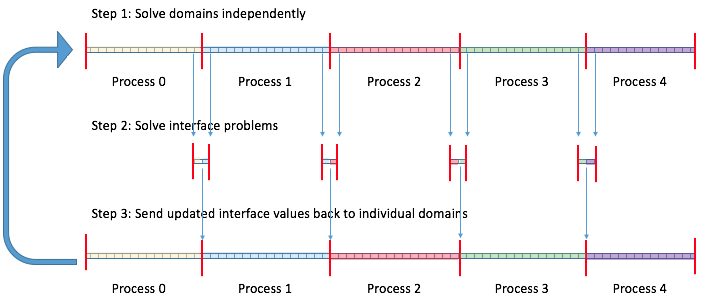
\includegraphics[width=0.8\textwidth]{../figures/1D-dd2.png}
\caption{Basic algorithm for 1-D domain decomposition using the interface problem method.}
\end{figure}

There are several possible algorithms for solving the interface problem. A master-slave approach can be taken, and a single process computes all interface problems. This is the natural approach in higher dimensions when the interfaces between the domains are connected (like the white regions on a giraffe). However, in 1-D, an alternative approach has each process communicate a single boundary condition value to its right neighbor. Then, the odd processes solve an interface problem, and communicate a single value back to its left neighbor. This approach can only be used when the interfaces are decoupled from each other, but offers greater potential for parallel efficiency since at least half of the processes are working during the interface solve, as opposed to a single process using the master-slave approach. In higher dimensions, the master-slave approach does not necessarily need to be used, and recursive domain decomposition could be applied to solve the interface problem using multiple MPI processes (but due to lack of time this is not pursued here).
\end{enumerate}

The interface problem method, where each domain communicates with at most two other domains (its left and right neighbors), is pursued in this project. This reduces the number of broadcast operations required and also has the potential to reduce overall runtime because each processor at most communicates with two other processors and only half of the processes are idle during the interface solve (unless communication is overlapped with computation using nonblocking communications). 

The pseudo code for this parallel implementation differs little from the pseudo code the serial version, except that extra pre-processing steps are necessary to divide the domain into as-close-as-possible equal-sized domains and prescribe initial guesses for the domain interface boundary conditions. Then, in a while loop, the processes solve their domains individually, send a boundary condition to their right, and wait to receive an updated boundary condition from their right neighbor after that process solves the interface problem. The following pseudo code shows the MPI implementation of the iterative domain decomposition algorithm (with some details omitted). Because the Poisson equation transmist information at infinite speeds, convergence of the domain decomposition algorithm fundamentally has to be based on the errors computed at {\it all} interfaces. That is, processes cannot finish in less iterations than some other process, since the problem is inherently global (unlike convection problems, where information travels at finite speeds). Hence, a barrier is required before beginning the next iteration loop. An iteration tolerance of 0.00001 is used for all results shown in this report.

\begin{lstlisting}
! divide problem into domains and assign to processes ...

do while (itererror > ddtol) ! iteration loop 
  ! save the previous values of the interface BCs
  prev = dd(rank + 1)%BCvals

  ! each processor solves for its domain --------------------------------------
  dd(rank + 1)%rglob(dd(rank + 1)%BCs(1)) = dd(rank + 1)%BCvals(1)
  dd(rank + 1)%rglob(dd(rank + 1)%BCs(2)) = dd(rank + 1)%BCvals(2)

  dd(rank + 1)%a = conjugategradient(rows, dd(rank + 1)%a, dd(rank + 1)%rglob, &
                                     dd(rank + 1)%BCs, reltol=reltol)

  ! each processor sends a boundary value to the processor to the right -------
  if (rank /= numprocs - 1) then
    call mpi_send(dd(rank + 1)%a(dd(rank + 1)%n_nodes - 1), 1, mpi_real8, &
                  rank + 1, rank, mpi_comm_world, ierr)
  end if

  ! processor to the right receives the message -------------------------------
  if (rank /= 0) then
    call mpi_recv(BClocals(1), 1, mpi_real8, rank - 1, rank - 1, &
                           mpi_comm_world, stat, ierr)
    BClocals(2) = dd(rank + 1)%a(2)
  end if

  call mpi_barrier(mpi_comm_world, ierr)

  ! each processor solves its interface problem -------------------------------
  if (rank /= 0) then
    dd(rank + 1)%BCvals(1) = (rel(2) + rel(1) - kel(2, 1) * BClocals(2) &
                      - kel(1, 2) * BClocals(1)) / (kel(2, 2) + kel(1, 1))
    ! send new interface result to rank - 1 process (to BCvals(2) of rank - 1)
    call mpi_send(dd(rank + 1)%BCvals(1), 1, mpi_real8, rank - 1, rank, &
                           mpi_comm_world, ierr)
  end if

  ! rank - 1 process receives from the process to the right -------------------
  if (rank /= numprocs - 1) then
    call mpi_recv(dd(rank + 1)%BCvals(2), 1, mpi_real8, rank + 1, rank + 1, &
                  mpi_comm_world, stat, ierr)
  end if

  ! compute iteration error to determine whether to continue looping ----------
  call mpi_allreduce(abs(dd(rank + 1)%BCvals - prev), itererror, 1, mpi_real8, &
                                mpi_sum, mpi_comm_world, ierr)

  call mpi_barrier(mpi_comm_world, ierr)
  ddcnt = ddcnt + 1
end do ! ends outermost domain decomposition loop
\end{lstlisting}

The pre-processing step of computing domain decomposition information such as the domain edge points and initial boundary condition values, are computed (redundantly) by {\it every} process. This eliminates communication from a single process to all other processes of this information, which would be more costly than simply having every process recompute the same information (since this portion of the algorithm accounts for a negligibly small fraction of the total run time). Because the cost of a matrix-vector product is roughly \(\mathscr{O}(N)\), the cost of the CG solver is \(I\mathscr{O}(n)\), where \(I\) is the number of CG iterations required. Likewise, the relative cost of a domain decomposition iteration is of order \(ID\mathscr{O}(N)\), where \(D\) is the number of domain decomposition iterations required for all processes to agree on the values of the solution at the interfaces. Hence, the success of the parallel implementation absolutely requires relatively few iterations amongst processes. This important feature will be returned to shortly.

Several interesting observations resulted from this initial implementation. The solution over the domain, given a constant heat source and thermal conductivity, will be parabolic. But, assuming we don't know this information, an initial guess for the interface boundary conditions was selected by assuming a straight-line solution between the two endpoints. Iterative global solutions are plotted in Fig. \ref{fig:interface}(a) for boundary conditions of 2 on the left and 3 on the right for 5 MPI processes for an interface width of two elements (i.e. each interface problem solves a 2-element domain, centered on the boundary between the decomposed domains). Each dashed line represents an domain decomposition iteration (where interface BCs are updated between each iteration), with only every 20 iterations shown. With this initial boundary condition guess, 1017 domain decomposition iterations are required! This is more than double the number of elements, and additional tests show that it increases with the number of elements. This number of iterations is far too large, so some steps must be taken to improve the algorithm to reduce the number of iterations.

The first approach taken to reduce the total number of domain decomposition iterations was to used a wider interface problem. That is, the width of each processor domain becomes smaller, and the interface region becomes wider. It was hoped that this would lead to faster convergence, because as can be seen in Fig. \ref{fig:interface}(a), because the solution values one element apart from the domain interfaces are very close to each other in magnitude, the interface values change with correspondingly small magnitude each iteration. With a wider interface, the boundary values for each interface are more different from each other, which could lead to faster convergence. Results obtained for the same problem characteristics, but with an interface width of 10 elements, is shown in Fig. \ref{fig:interface}(b). With this wider interface, only 234 domain decomposition iterations are required, but the solution obtained is now incorrect (as assessed by comparing to the analytical solution). This occurs because the larger the interface, the greater the magnitude of the error in the initial boundary condition guesses (because the straight-line solution is incorrect), and choosing a wider interface applies this error over a wider range. For this particular example, this results in a sharp corner developing in the solution. This interesting result shows that the interface region must be kept very small. 

\begin{figure}[H]
        \centering
        \begin{subfigure}[b]{0.5\textwidth}
                \centering
                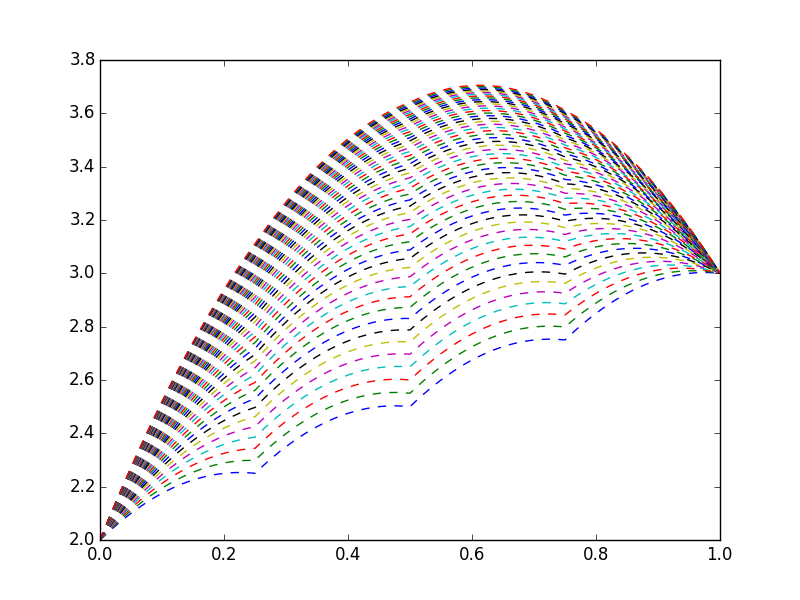
\includegraphics[width=\textwidth]{../figures/interface1.png}
                \caption{Interface width of 2 elements}
        \end{subfigure}%
                \begin{subfigure}[b]{0.5\textwidth}
                \centering
                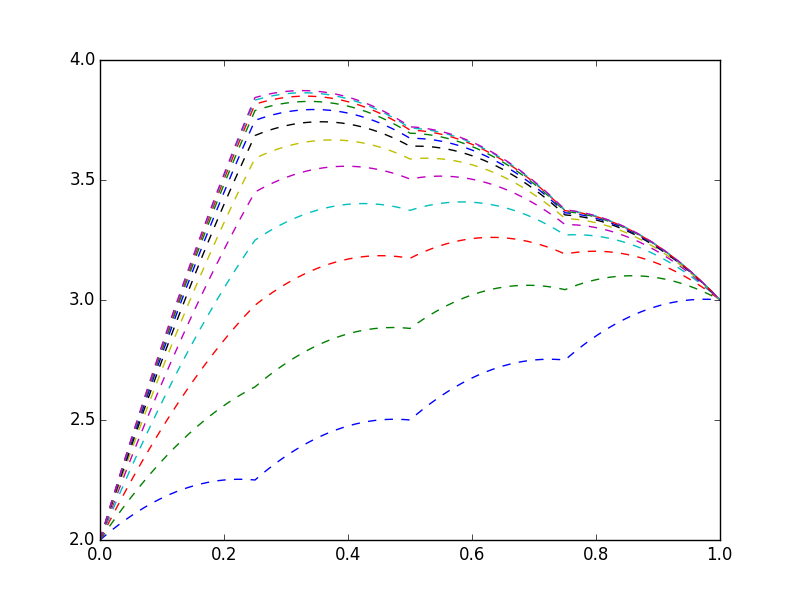
\includegraphics[width=\textwidth]{../figures/interface2.png}
                \caption{Interface width of 10 elements}
        \end{subfigure}%
        \caption{Iterative solutions (only every 20 iterations are plotted) for (a) an interface width of 2 elements and (b) an interface width of 10 elements for 5 MPI processes, 500 elements, and initial interface boundary condition values given by a straight line between the two endpoints.}
\label{fig:interface}
\end{figure}

If the interface region is to be kept so small, then some other algorithmic change must be done to reduce the number of domain decomposition iterations. The next approach taken was to improve the initial boundary conditions guesses by solving a coarse-mesh problem. The rank 0 process solves a coarse mesh solution, where the mesh nodes are taken as the nodes on the domain interfaces. For a 5-process solve, the coarse mesh would consist of 5 elements, with nodes at the same locations as the domain interfaces. After the rank 0 process computes this solution (the algorithm for which is identical to the larger solves, but with fewer elements), the better interface initial conditions are broadcast to all other processes, and then every process continues with the domain decomposition algorithm described earlier. This change produced a {\it huge} improvement. For the same iteration tolerance used for the results in Fig. \ref{fig:interface}, only one domain decomposition iteration is required! Hence, a major take-away from this project that wasn't touched upon by our homework assignments is that parallel implementations that require iteration amongst processes can easily be fundamentally slower than serial implementations (not just because of communication overhead, but rather the requirement of {\it more} iterations). For this project, the use of this better inter-processor initial condition was used to yield a successful implementation. In practice, many codes that use domain decomposition will perform a coarse mesh solution that is also used for preconditioning to further enhance the parallel viability of an iterative domain decomposition method.

After obtaining a working MPI implementation, OpenMP parallelism was added at a fine-grained level to all parallelizable loops. 








\subsection{Alternative Parallel Implementations}
This section briefly discusses several alternative parallel implementations that were pursued early-on in the project before determining that the interface problem approach described previously was the best option. The overlapping Schwarz method, where only half of the domains can be solved at any one time, proved to be too slow, since at any one time about half of the processes are idle. However, this approach did not require any interface solves. But with an interface of width 2 elements, the cost of the interface solves is negligible, and hence the dominant feature of idle processes proved this approach to be too slow. The code for this implementation is shown in the Appendix as {\tt amain.f90}, but for brevity none of the results are discussed except to say that the method was much slower than the chosen method. At any one time, the interface problem approach, where each process except the rank 0 process computes an interface problem, {\it at most} has a single process idle.

\section{Implementation Results}
This section discusses implementation results with the serial, MPI, and MPI plus OpenMP implementations. To keep things fair, the serial case uses the same initial condition as the MPI cases, and a number of ``pretend processes'' are passed on the command line to the serial case to compute the coarse mesh initial conditions (which is then input as a whole to the CG solver). When using the same initial condition, the serial and parallel implementations perform almost the same number of cumulative CG iterations (because with the better initial condition only one domain decomposition iteration is needed), the only difference being that for the parallel implementations, each process performs a subset of the iterations. First, results will be shown for the implementation of sole MPI parallelism to determine the speedup relative to serial and the strong and weak scaling. Then, results will be shown of the combined MPI-OpenMP parallelism to determine the added performance associated with the use of OpenMP.





Fig. \ref{fig:speedupMPI}(a) shows the speedup achieved for 2 to 24 MPI processes on a single node on Edison. The raw data used to generate this plot is shown in Fig. \ref{fig:speedupMPIruntime}(a), where it is shown that the serial runtime is relatively constant for a given number of elements, but the parallel implementation runtime decreases with the number of processes. Because the total number of CG iterations is roughly proportional to the number of elements, but not the number of processes, this substantial difference in runtime can be attributed to the {\it overall} algorithm {\it not} scaling as \(\mathscr{O}(N)\), but rather as some higher power of \(N\), since then the impact of reducing the number of elements per solve has a greater and greater impact (because the speedup increases better than linearly). However, the results shown for a single node are not entirely useful, since rarely would you run as many as 24 MPI processes on a single node - a more common number is between 1 and 4 MPI processes per node. To test how the runtime is affected by the partitioning of MPI processes among nodes, the same simulation is run with 12 compute nodes and between 1 and 8 MPI processes per node. The raw data is shown in Fig. \ref{fig:speedupMPIruntime}(b), and the speedup in Fig. \ref{fig:speedupMPI}(b) for the optimal selection of xxxx MPI processes/node.

\begin{figure}[H]
        \centering
        \begin{subfigure}[b]{0.5\textwidth}
                \centering
                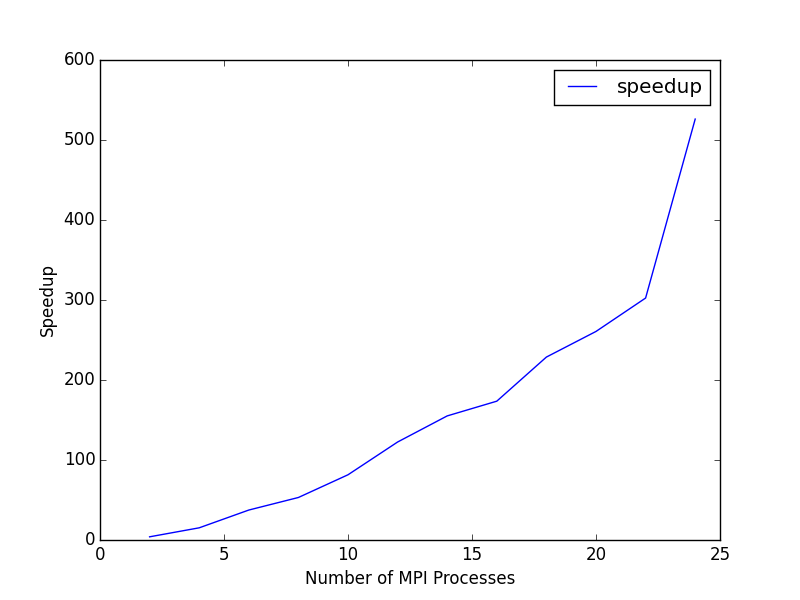
\includegraphics[width=\textwidth]{../figures/speedup-mpi.png}
                \caption{Single node}
        \end{subfigure}%
                \begin{subfigure}[b]{0.5\textwidth}
                \centering
                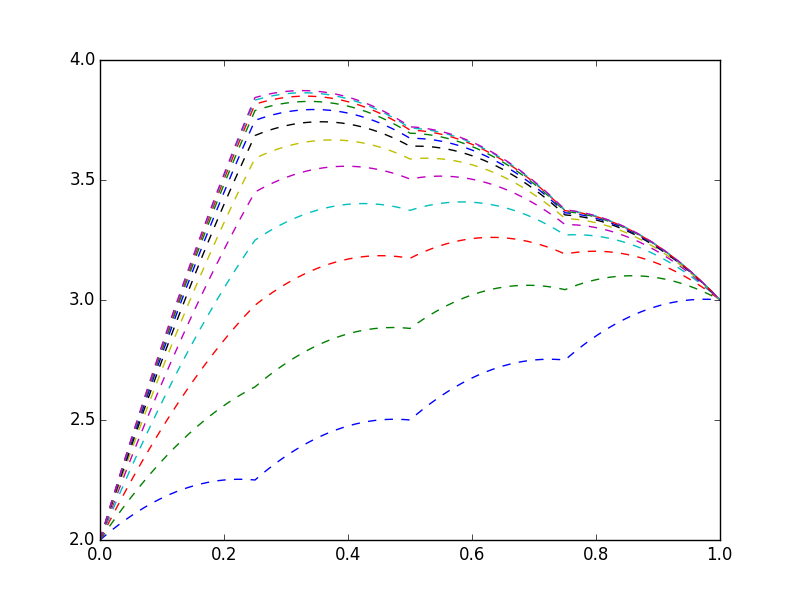
\includegraphics[width=\textwidth]{../figures/interface2.png}
                \caption{12 nodes}
        \end{subfigure}%
\caption{Speedup relative to serial performance as a function of the number of MPI processes on (a) a single node for 20,000 elements, and (b) 12 nodes with 100,000 elements using xxxx MPI processes/node. Note that because the initial condition depends on the number of processes, each data point is normalized to the speedup using that number of ``pseudo'' processes. To avoid wasting computing resources, and because the runtime for the serial algorithm is approximately independent of the initial condition guess, the speedup for (b) is normalized to the serial runtime for 96 pseduo-processes (since this would be the best runtime anyways, this is conservative).}
        \label{fig:speedupMPI}
\end{figure}


\begin{figure}[H]
        \centering
        \begin{subfigure}[b]{0.5\textwidth}
                \centering
                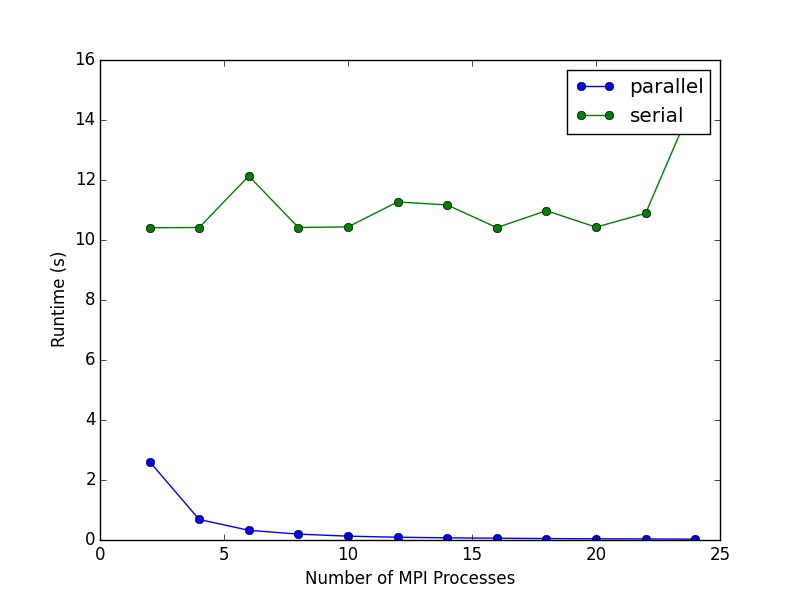
\includegraphics[width=\textwidth]{../figures/singlenode-mpi.png}
                \caption{Single node}
        \end{subfigure}%
                \begin{subfigure}[b]{0.5\textwidth}
                \centering
                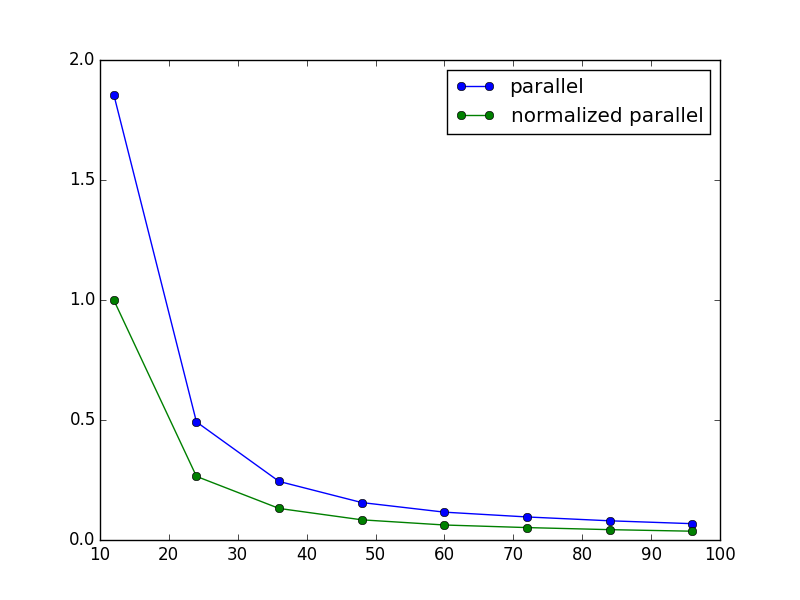
\includegraphics[width=\textwidth]{../figures/speedup-mpi-multinode.png}
                \caption{12 nodes}
        \end{subfigure}%
\caption{Runtime as a function of the number of MPI processes on (a) a single node for 20,000 elements, and (b) 12 nodes with 100,000 elements.}
        \label{fig:speedupMPIruntime}
\end{figure}








\section{Appendix}
\subsection{Details of the Finite Element Method}
This section contains additional discussion of the FEM that is necessary to fully understand the code developed, but not necessary to appreciate parallelization algorithms.

\subsubsection{The Element-Wise Weak Form}
The stiffness matrix shown in Eq. \eqref{eq:Stiffness} consists of the multiplication of the derivatives of \(\phi_i(x)\) with \(\phi_j(x)\). If these shape functions are defined over the {\tt entire} domain, then the stiffness matrix will be a dense matrix. On the other hand, if we choose these shape functions to be nonzero only over a single small region of the domain, then the product of cross terms will be zero for most of the matrix, since the effect of a single shape function will be very localized. This will produce sparse matrices, which will be much easier to work with and will also permit easier extension as a numerical method over a discretized domain. Hence, the expansion for the solution and test function for a {\it single} element (``element'' is used in this sense as a small region of the domain, i.e. a meshing software would divide up a continuous domain into discrete elements) becomes:

\beq
T_h^e=\sum_{j=1}^{n_{en}}c_j^e\phi_j^e(x)
\eeq

where the \(e\) superscript indicates the element and \(n_{en}\) are the number of element nodes. A nodal basis is selected for the shape functions. This means that, over a single element, the shape functions are unity at their corresponding node, and zero at the other nodes. The matrix equation \(K_{ij}c_j=R_i\) can be written for written for each individual element, with a post-processing step that takes the system of equations for each element and connects them all together to enforce solution continuity at element interfaces. 

\beq
K_{ij}^ec_j^e=R_i^e
\eeq

where

\beq
K_{ij}^e=\int_{\Omega^e}\frac{\partial \phi_j(x)}{\partial x}k\frac{\partial\phi_i(x)}{\partial x}dx-\int_{\Gamma^e}k\frac{\partial \phi_j(x)}{\partial x}\phi_i(x)\cdot\hat{n}dx
\eeq

\beq
R_{i}^e=\int_{\Omega^e}\dot{q}\phi_i(x)dx
\eeq

such that the domain of integration is only over a single element. However, the system of equations for each element, \(K_{ij}^ec_j^e=R_i^e\), is singular, and cannot be solved independently of the other elements, since we require solution continuity at inter-element nodes. This requires the formation of a connectivity matrix.

\subsubsection{The Connectivity (Location) Matrix}
Figure \ref{fig:FEmesh} shows a simple FE mesh, where the numbers illustrate the global node numbering. A mapping is required from the elemental perspective to this global mesh. The location matrix contains this information - each column of the location matrix gives the global node numbers that correspond to the local node numbers. The local nodes must always be numbered in a consistent manner (i.e. always clockwise or always counterclockwise) so that the Jacobian of the local to global transformation is positive. The first five columns of the location matrix for this mesh, for illustration, would be:

\beq
\label{eq:LM}
LM=\begin{bmatrix}
1 & 2 & 3 & 4 & 5 & \cdots\\
2 & 3 & 4 & 5 & 6 & \cdots\\
11 & 12 & 13 & 14 & 15 & \cdots\\
10 & 11 & 12 & 13 & 14 & \cdots\\
\end{bmatrix}
\eeq

where the nodes have been numbered counterclockwise.

\begin{figure}[H]
\centering
\includegraphics[width=0.8\textwidth]{../figures/FEmesh.pdf}
\caption{Global node numbering in a simple FE mesh. Source:\newline {\tt http://opensees.berkeley.edu/wiki/index.php/}\newline{\tt Simply\_supported\_beam\_modeled\_with\_two\_dimensional\_solid\_elements}}
\label{fig:FEmesh}
\end{figure}

For structured meshed, this location matrix is fairly easy to determine, but for unstructured meshes where there is not necessarily a pattern to the node connectivity, would be provided by a meshing software such as Cubit.  Once this location matrix is known, the elemental systems of equations \(K_{ij}^ec_j^e=R_i^e\) can be assembled into the global system of equations \(K_{ij}c_j=R_i\). The fundamental reason why it is preferred to assemble the equations for each element individually, and {\tt then} assemble these into a global system, is that we have chosen shape functions that are only nonzero over an element and its immediate neighbors. This algorithm is inherently local until we get to the step requiring continuity, and it is hence natural to avoid unnecessary computations of zero integrals by only computing the integrals over each element, and then assembling these systems together at the end right before the numerical solve. For better illustration, several entries of \textbf{K} are assembled as follows for the location matrix given in Eq. \eqref{eq:LM}.

\beqa
K(1, 1) =& k(1, 1)^{e=1}\\
K(1, 2) =& k(1, 2)^{e=1}\\
K(2, 2) =& k(2, 2)^{e=1}+k(1, 1)^{e=2}\\
K(2, 11) =& k(2, 3)^{e=1}\\
K(12, 12) =& k(3, 3)^{e=2}+k(4, 4)^{e=3}\\
\eeqa

where a new notation of lowercase \(k\) representing \(K^e\) is used.

\subsubsection{Boundary Conditions}
Once the global matrix has been assembled, any Dirichlet boundary conditions must be applied (Neumann boundary conditions have naturally been applied by the form of the perimeter integral in Eq. \eqref{eq:k}). Dirichlet boundary conditions are strictly imposed by removing the Dirichlet nodes from the global matrix system. For a 1-D domain consisting of four linear elements (two nodes per element), the global matrix system \(\textbf{K}c=\textbf{R}\) before imposition of Dirichlet boundary conditions is:

\beq
\textbf{K}=
\begin{bmatrix}
k(1, 1)^{e=1} & k(1, 2)^{e=1} & 0 & 0 & 0\\
k(2, 1)^{e=1} & k(2, 2)^{e=1}+k(1, 1)^{e=2} & k(1, 2)^{e=2} & 0 & 0\\
0 & k(2, 1)^{e=2} & k(2, 2)^{e=2}+k(1, 1)^{e=3} & k(1, 2)^{e=3} & 0\\
0 & 0 & k(2, 1)^{e=3} & k(2, 2)^{e=3}+k(1, 1)^{e=4} & k(1, 2)^{e=4}\\
0 & 0 & 0 & k(2, 1)^{e=4} & k(2, 2)^{e=4}\\
\end{bmatrix}
\eeq

\beq
\textbf{R}=\begin{bmatrix}
R_1^{e=1} \\ R_2^{e=1}+R_1^{e=2}\\R_2^{e=2}+R_1^{e=3}\\R_2^{e=3}+R_1^{e=4}\\R_2^{e=4}\\
\end{bmatrix}
\eeq

To apply Dirichlet boundary conditions at nodes \(1\) and \(5\), the off-diagonal terms in the stiffness matrix are set to zero and the corresponding terms in the global load vector are set to the Dirichlet values. For instance, to impose Dirichlet conditions of \(T(node 1)=3.5\) and \(T(node 5) = 10.5\), the global matrix system becomes:

\beq
\textbf{K}=
\begin{bmatrix}
1 & 0 & 0 & 0 & 0\\
k(2, 1)^{e=1} & k(2, 2)^{e=1}+k(1, 1)^{e=2} & k(1, 2)^{e=2} & 0 & 0\\
0 & k(2, 1)^{e=2} & k(2, 2)^{e=2}+k(1, 1)^{e=3} & k(1, 2)^{e=3} & 0\\
0 & 0 & k(2, 1)^{e=3} & k(2, 2)^{e=3}+k(1, 1)^{e=4} & k(1, 2)^{e=4}\\
0 & 0 & 0 & 0 & 1\\
\end{bmatrix}
\eeq

\beq
\textbf{R}=\begin{bmatrix}
3.5\\ R_2^{e=1}+R_1^{e=2}\\R_2^{e=2}+R_1^{e=3}\\R_2^{e=3}+R_1^{e=4}\\10.5\\
\end{bmatrix}
\eeq

\section{The Conjugate Gradient Method}
The CG method requires computation of the residual:

\beq
r^i=R-\textbf{K}a^i
\eeq

where \(i\) is the iteration index.Each update to the solution iterates is performed according to:

\beq
\label{eq:CGUpdate}
a^{i+1}=a^i+\lambda^iz^i
\eeq

where the update scales by \(z^i\):

\beq
\label{eq:ZUpdateCG}
z^i=r^i+\theta^iz^{i-1}
\eeq

where \(\theta^i\) is a parameter chosen such that \(z^i\) is \(\textbf{K}\)-conjugate to \(z^{i-1}\), or:

\beq
\label{eq:kconjugate}
z^{T,i}\textbf{K}z^{i-1}=0
\eeq

In other words, the search direction is a combination of a move in the reverse direction of the gradient (method of steepest descent) plus a motion perpendicular to that direction. This helps to avoid duplicate searching in the same general area. For the very first iteration, it is common to select \(z^1=r^1\). Simply plugging in Eq. \eqref{eq:ZUpdateCG} to Eq. \eqref{eq:kconjugate} gives:

\beq
\theta^i=-\frac{r^{T,i}\textbf{K}z^{i-1}}{z^{T,i-1}\textbf{K}z^{i-1}}
\eeq

Plugging in Eq. \eqref{eq:CGUpdate} into Eq. \eqref{eq:IterativeMethodsPotential} and then taking the partial derivative with respect to \(\lambda^i\), the optimal \(\lambda^i\) is:

\beq
\label{eq:UpdateCG}
\lambda^i=\frac{z^{T,i}r^i}{z^{T,i}\textbf{K}z^i}
\eeq

\end{document}
